\documentclass[a4paper]{article}

\usepackage[spanish]{babel}
\usepackage[utf8]{inputenc}
\usepackage{amsmath}
\usepackage{graphicx}
\usepackage[colorinlistoftodos]{todonotes}
\usepackage{multicol}
\usepackage{makeidx}
\usepackage{hyperref}
\usepackage{caption}
\usepackage{amsfonts}
\usepackage{amssymb}
\usepackage{amsmath}
\usepackage[utf8]{inputenc}
\usepackage{verbatim}
\usepackage{listings}
\usepackage{algpseudocode}
\usepackage{courier}
\usepackage{enumitem}
\usepackage{placeins}



\newcommand{\BigO}[1]{\ensuremath{\operatorname{O}\bigl(#1\bigr)}}
\lstset{language=C++, showstringspaces=false, tabsize=2, breaklines=true, title=\lstname}

\usepackage{booktabs}
\usepackage[margin=1in]{geometry}

\title{Trabajo Práctico I de Teoría de las Comunicaciones}

\author{, Nicolás Lasso, , }

\date{\today}

\makeindex

\begin{document}
\newgeometry{margin=2cm}
\pagenumbering{gobble}
\raggedleft

\includegraphics[width=8cm]{caratula/logo1.jpg}\\

\raggedright
\vspace{3cm}
{\Huge \bfseries Trabajo Práctico 1}
\rule{\textwidth}{0.02in}
\large Miércoles 29 de abril de 2015 \hfill Teoría de las Comunicaciones
\vspace{1.5cm}

\normalsize
\begin{tabular}{|l@{\hspace{5ex}}c@{\hspace{5ex}}l|}
        \hline
        \rule{0pt}{1.2em}Integrante & LU & Correo electrónico\\[0.2em]
        \hline
        \rule{0pt}{1.2em} Nahuel Lascano  & 476/11 &\tt laski.nahuel@gmail.com\\[0.2em]
		\rule{0pt}{1.2em} Nicolás Lasso & 763/10 &\tt lasso.nico@gmail.com\\[0.2em]
        \rule{0pt}{1.2em} Roberto Rama  & 490/11 &\tt bertoski@gmail.com\\[0.2em]
        \rule{0pt}{1.2em} Pablo Somodi  & 818/10 &\tt psomodi@dc.uba.ar\\[0.2em]
        \hline
\end{tabular}

\vspace{1.0cm}
\raggedright

\begin{multicols}{2}

\includegraphics[width=8cm]{caratula/logo-uba.png}

\columnbreak
\vspace*{4.5cm}
\raggedleft
\textbf{Facultad de Ciencias Exactas y Naturales}\\
Universidad de Buenos Aires\\
\small
Ciudad Universitaria - (Pabellon I/Planta Baja)\\
Intendente G\"uiraldes 2160 - C1428EGA\\
Ciudad Autonoma de Buenos Aires - Rep. Argentina\\
Tel/Fax: (54 11) 4576-3359\\
http://www.fcen.uba.ar
\end{multicols}

\restoregeometry

\clearpage

\pagenumbering{arabic}

\tableofcontents

\vspace{3cm}

\clearpage

\setlength{\parindent}{10pt}

\section{Introducción}
En el presente trabajo práctico tuvimos como desafío implementar una herramienta muy común de diagnóstico de red, el traceroute.

Por medio de la misma los administradores de red pueden analizar la ruta que sigue un paquete hasta un destino dado.

Los fundamentos de dicha herramienta son muy sencillos.
Se utilizan paquetes IP para recorrer la ruta aumentando de un salto a la vez.
Esto se hace por medio del campo TTL (\textit{Time to live}) que nos permite configurar la cantidad máxima de ``saltos'' que se le permiten al paquete para llegar a destino.
Cuando un router recibe un paquete para redireccionarlo, previo a esto decrementa en 1 su TTL, si el mismo resulta igual a 0 entonces devuelve el mensaje \textbf{ICMP Time Exceeded} a la dirección de origen.

La herramienta se basa en este comportamiento para obtener la información de la ruta. La misma envía varios paquetes incrementando el TTL progresivamente desde 1 hasta que el paquete efectivamente llega a destino, y va registrando los paquetes de respuesta \textbf{ICMP Time Exceeded} que recibe de cada router.

Esta herramienta se puede implementar con paquetes ICMP, TCP o UDP, según necesidad. La herramienta default que se ofrece en cualquier distribución de Linux permite realizar el procedimiento con los tres tipos de paquetes.

\clearpage

\section{Capturando tráfico}
Para poder entender el trabajo que hicimos es preciso en primer lugar comprender
el funcionamiento del protocolo ARP. El protocolo se utiliza para averiguar a
qué dirección MAC corresponde una dirección IP determinada dentro de una red. El
nodo que quiere averiguar esta información hace un broadcast Ethernet de un
paquete ARP ``who-has'' con la dirección IP a consultar, y alguno de los nodos
de la red que tenga la respuesta en su tabla ARP le envía un paquete ARP
``is-at'' con la dirección MAC correspondiente.

La herramienta que desarrollamos captura los paquetes Ethernet que circulen en la red mediante el comando \textit{sniff()} del paquete Scapy.
Por cada paquete guardamos su campo ``type'' y su tamaño, para luego poder calcular la fuente $S$ y el overhead impuesto por el protocolo ARP.
Además, para los paquetes ARP en particular guardamos los siguientes datos: la IP destino (de qué dispositivo se quiere averiguar la MAC), la IP origen (qué dispositivo es el que quiere averiguarla), y el tipo de paquete (who-has o is-at).

El primer desafío fue elegir el campo de los paquetes ARP a usar como fuente $S_1$. Las posibilidades eran:
\begin{itemize}
	\item Quién emite un paquete who-has (\textit{who-has-src})
    \item Por quién pregunta un paquete who-has (\textit{who-has-dst})
    \item Quién responde un paquete is-at (\textit{is-at-src})
    \item A quién le responde un paquete is-at (\textit{is-at-dst})
\end{itemize}

Para elegirla, realizamos las capturas y analizamos la información obtenida en cada caso. Eso nos llevó a elegir \textit{who-has-dst}. Descartamos ambos \textit{is-at} porque en las redes cableadas no veíamos practicamente tráfico de estos paquetes (solo los emitidos y los respondidos por la propia computadora que realizaba las capturas) dado que por defecto no se \textit{floodean}. Dentro de los (\textit{who-has}), preferimos ver por quién se pregunta, por ser en general más consistente con nuestro conocimiento sobre las redes analizadas (al parecer, algunos nodos preguntan bastante comparativamente, por más que no sean particularmente relevantes en la red).

Como requería el trabajo, implementamos una herramienta para capturar paquetes y realizamos capturas en cuatro puntos distintos: los laboratorios del Departamento de Computación, la biblioteca del Pabellón 2, un Starbucks ubicado en Av. Cabildo y Juana Azurduy y la casa de uno de los integrantes.


%ME FALTA EL CÁLCULO DE ENTROPÍA DE LAS FUENTES.

\clearpage

\section{Resultados y análisis}
% EN LA PRIMERA CONSIGNA YO HABLO DE QUÉ CAMPO ELEGIMOS Y POR QUÉ (DEST DEL WHO-HAS). LA IDEA ES QUE ACÁ HABLEN DE LAS CAPTURAS, DETERMINANDO LOS NODOS DISTINGUIDOS DE CADA UNA DE LAS REDES, PEGANDO LOS GRÁFICOS (TORTA Y BARRITAS).

% APARTE, AL FINAL, ESTARÍA BUENO HABLAR DE CASOS "RAROS", COMO EL GRÁFICO DONDE 0.0.0.0 APARECE COMO EMISOR.

\subsection{Entropía de la fuente $S$}
En las cuatro capturas que realizamos la fuente planteada en el enunciado (el campo \textit{type} de capa 2) tenía una fuerte inclinación hacia los paquetes de tipo IPv4, por razones obvias: el protocolo IPv6 aún no goza de suficiente difusión y todas las redes que usamos se usaban principalmente para trabajar en Internet.

Esto dio como resultado una entropía bastante baja en esta fuente, siendo la más alta 0,93621 que corresponde a las aulas de computación de la Biblioteca del Pabellón 2, y la más baja 0,11652 que corresponde a la casa de uno de los integrantes del grupo.

\subsection{Entropía de la fuente $S_{1}$}
En este caso los valores cobran más interés, pues al tener en cuenta los destinatarios de los paquetes \textit{who-has} hay, en general, mayor cantidad de símbolos. La fuente de mayor entropía fue, una vez más, la de la Biblioteca del Pabellón 2, con un valor aproximado de 6,76823, seguida de cerca por los Laboratorios del DC con 5,40519. La de menor entropía fue la captura realizada en Starbucks, con un 2,88843.

Finalmente, para tener una mejor visualización de los datos obtenidos, decidimos
utilizar diferentes gráficos para sintetizar y presentar la información que
consideramos más relevante de las redes analizadas.

\subsection{Estadísticas}
\subsubsection{Cantidad de paquetes y tiempos de captura}

\begin{table}[h]
\centering
\begin{tabular}{@{}cccc@{}}
\toprule
Red                     & Cantidad ARP & Cantidad otros & Tiempo \\ \midrule
Aulas Pabellon 2        & 4852         & 16757          & 60min      \\
Laboratorios Pabellon 1 & 309          & 42031          & 30min  \\
Starbucks               & 124          & 8890           & 30min  \\
Home LAN                & 113          & 43058          & 60min      \\ \bottomrule
\end{tabular}
\end{table}

\subsubsection{Entropía}
\begin{table}[h]
\centering
\begin{tabular}{@{}ccc@{}}
\toprule
Red                     & Fuente modelada $S$ & Entropia H($S$) \\ \midrule
Aulas Pabellon 2        & $S$              & 0.93621       \\
Aulas Pabellon 2        & $S_{1}$              & 6.76823       \\ \midrule
Laboratorios Pabellon 1 & $S$              & 0.12087       \\
Laboratorios Pabellon 1 & $S_{1}$              & 5.40519       \\ \midrule
Starbucks               & $S$              & 0.26268       \\
Starbucks               & $S_{1}$              & 2.88843       \\ \midrule
Home LAN                & $S$              & 0.11652       \\
Home LAN                & $S_{1}$              & 2.13766       \\ \bottomrule
\end{tabular}
\end{table}

\newpage
\subsection{Home LAN}
\begin{center}
	\begin{figure}[ht]
    	\centering
		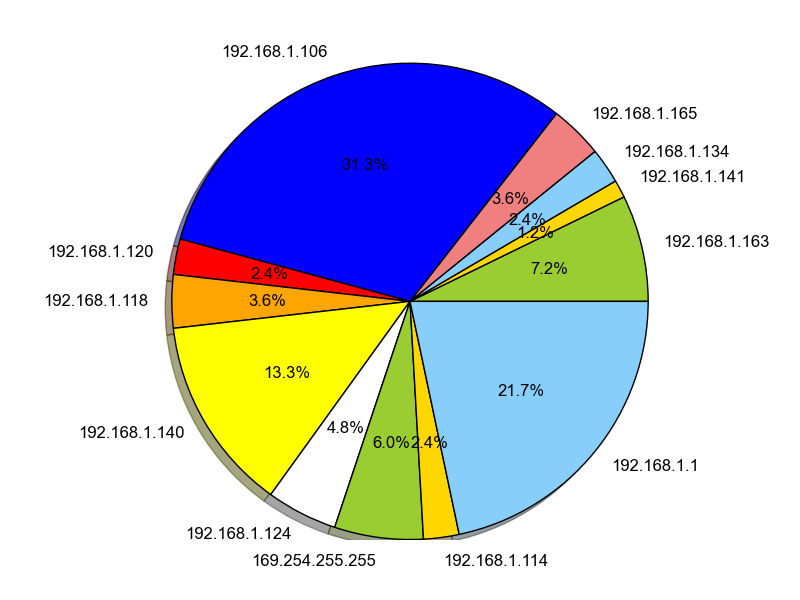
\includegraphics[width=12cm]{imgs/outputNicoLassoCasa_p-arp_who_dst-torta.png}
		\caption{Who-Has DST Red Nicolás Lasso}
	\end{figure}
\end{center}

\indent En la figura 1 se puede observar el volumen de tráfico de paquetes ARP who-has, agrupados por la ip de destino del paquete. 
Fueron capturados en una casa con varios dispositivos conectados, entre ellos Raspberry Pi, Apple TV, Televisiones y computadoras sin actividad. Ademas una sola persona se encontraba en ese momento conectada a la red con una computadora y un dispositivo Android. El dispositivo con la IP \textit{192.168.1.106}, uno de los más consultados, es una computadora personal. Luego también se encuentra con muchas consultas un dispositivo Android con la IP \textit{192.168.1.140}. Por último el dispositivo con IP \textit{192.168.1.1} es efectivamente el router como se verá más adelante.

\FloatBarrier
% \begin{center}
% 	\begin{figure}[ht]
%     	\centering
% 		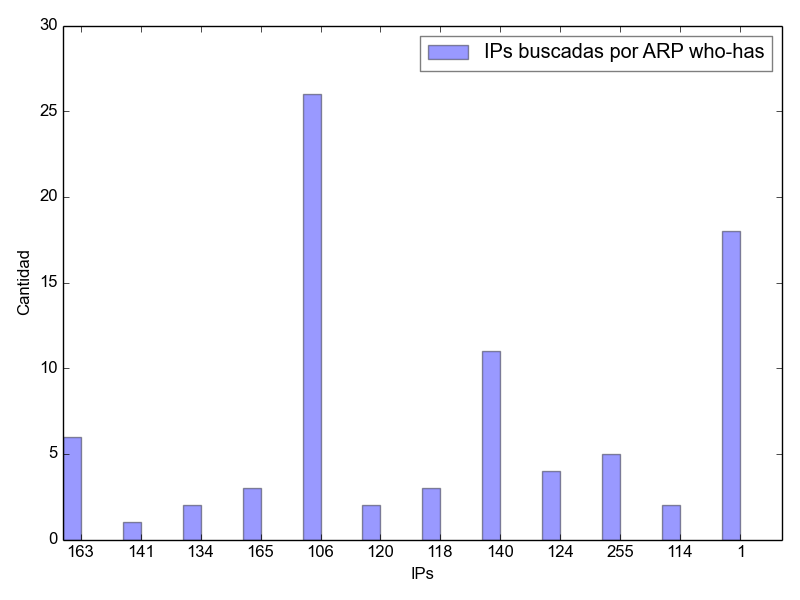
\includegraphics[width=10cm]{imgs/outputNicoLassoCasa_p-arp_who_dst.png}
% 		\caption{Who-Has DST Red Home}
% 	\end{figure}
% \end{center}
% \FloatBarrier

\FloatBarrier
\begin{center}
	\begin{figure}[ht]
    	\centering
		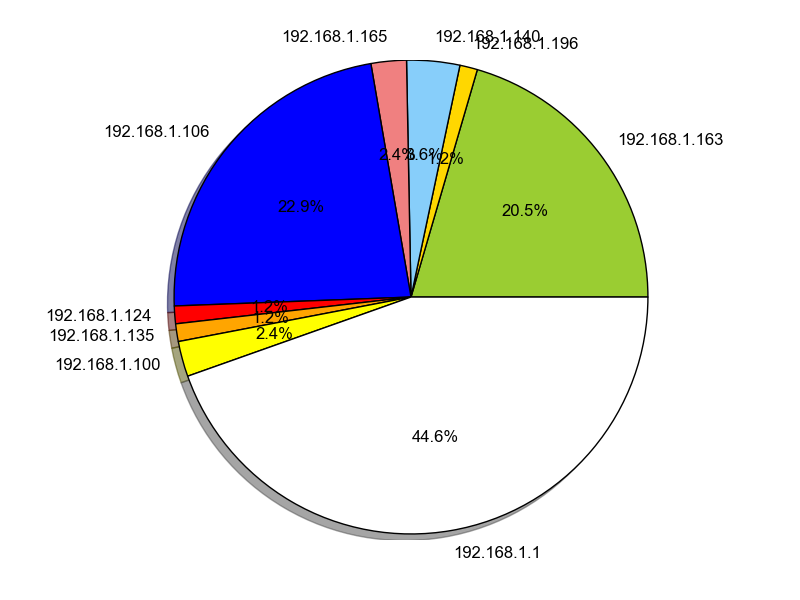
\includegraphics[width=10cm]{imgs/outputNicoLassoCasa_p-arp_who_src-torta.png}
		\caption{Who-Has SRC Red Home}
	\end{figure}
\end{center}
\FloatBarrier

\indent En esté gráfico se muestra que el nodo que más paquetes who-has envió fue efectivamente el Router con la IP \textit{192.168.1.1}. A continuación se encuentra un gráfico que muestra la cantidad de paquetes por cada tipo que fueron capturados:

\FloatBarrier
\begin{center}
	\begin{figure}[ht]
    	\centering
		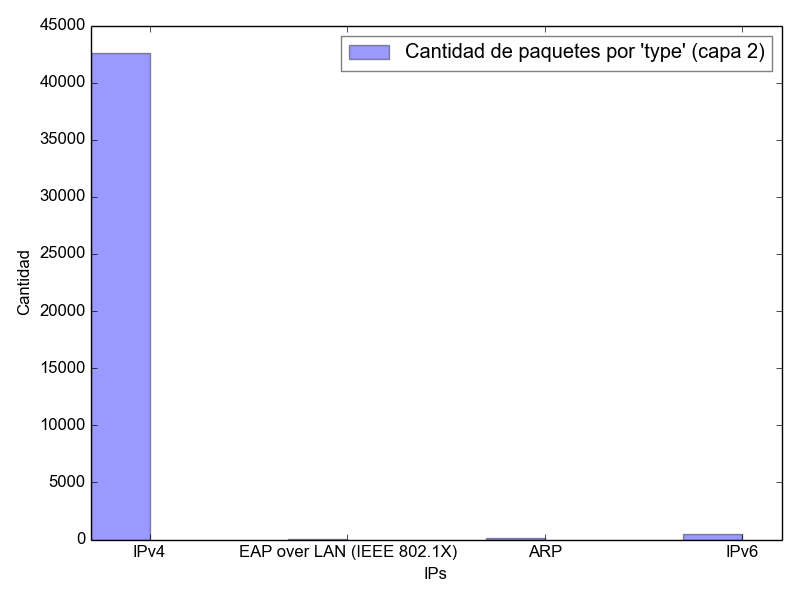
\includegraphics[width=10cm]{imgs/outputNicoLassoCasa_p-pkgs_by_type.png}
		\caption{Cantidad de Paquetes por tipo (Red Home)}
	\end{figure}
\end{center}
\FloatBarrier

\indent Se puede observar que los paquetes de tipo IPv4 son los que mayor cantidad muestran mientras que los paquetes de ARP tienen muy poca cantidad en comparación. Por otro lado se observa que los paquetes de tipo IPv6 son muy pocos aun ya que todavía no son muchos los nodos que se encuentran usando este tipo de protocolo.

\newpage
\subsection{LAN Aulas Biblioteca pabellón 2 \textit{FCEyN}}
\indent La siguiente Red se encuentra ubicada en las Aulas de la Biblioteca del pabellón 2. En la misma hay varias computadoras conectadas. La Herramienta se corrió en el router basado en Linux. A su vez es importante aclarar que dicho router se encontraba realizando NAT entre la red de backbone de la facultad (157.92.18.0) y la red de rango privado donde se encuentran los equipos de la sala de computación 10.221.0.99 \\
\indent A continuación se encuentran los gráficos que representan todas las capturas de los paquetes que fueron interceptados por la herramienta para ambas redes a las que pertenece el router.


\begin{center}
	\begin{figure}[ht]
    	\centering
		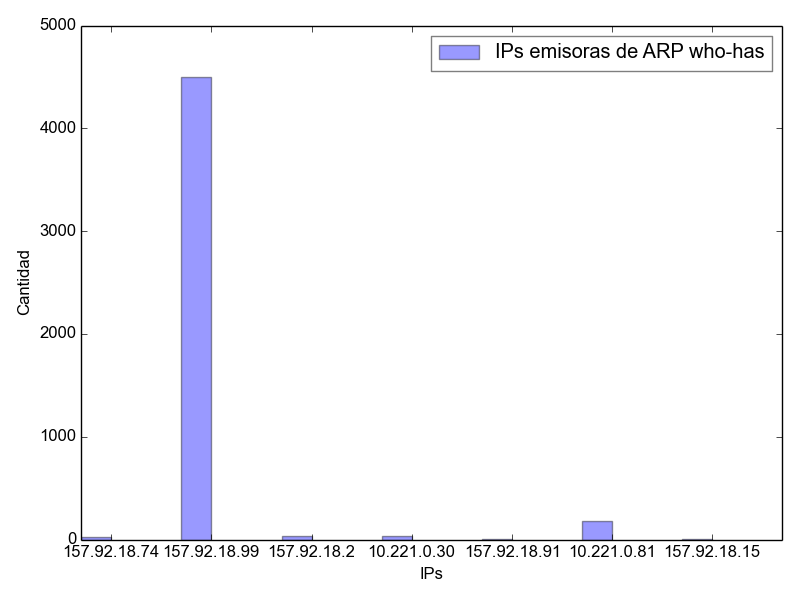
\includegraphics[width=12cm]{imgs/outputPabloRedAulasPab2_p-arp_who_src.png}
		\caption{Who-Has SRC Red Aulas Biblioteca del Pabellón 2 FCEyN}
	\end{figure}
\end{center}

Como se puede observar, el router de la red ``exterior'' (IP: 157.92.18.99) tiene una cantidad inmensamente superior de paquetes who-has emitidos.
Esto puede no solo ser producto de que sea el router de salida hacia internet desde donde nos encontrábamos corriendo la captura, sino también de que este router hace de gateway para varias redes diferentes que tienen un router ``intermedio'' en la red 157.92.18.0/24. Todas las búsquedas ARP que realizaba el 157.92.18.99 para encaminar tráfico hacia las subredes de la facultad fueron capturadas por nuestro experimento.

~

Adicionalmente se puede observar que una de las workstations de la sala de computación, con IP 10.221.0.81 se encontraba activa durante el momento de la captura y estaba generando tráfico ARP. 
Dado el horario de esta captura (fin de semana) asumimos que se trataba de actualizaciones del sistema operativo o algún proceso en background que generaba tráfico.

~

A su vez, se pudo observar un detalle interesante producto de que este equipo actúa de router entre dos redes.
Para el caso de paquetes ARP is-at, el origen de los paquetes emitidos por la captura fue siempre una IP del equipo: o bien la ``externa'' o bien la ``interna''. Sin embargo, lo extraño fue no observar ningún paquete is-at que lo enviara algún otro equipo con destino a este servidor (recordando que los paquetes is-at no se envían a toda la red).


\begin{center}
	\begin{figure}[ht]
    	\centering
		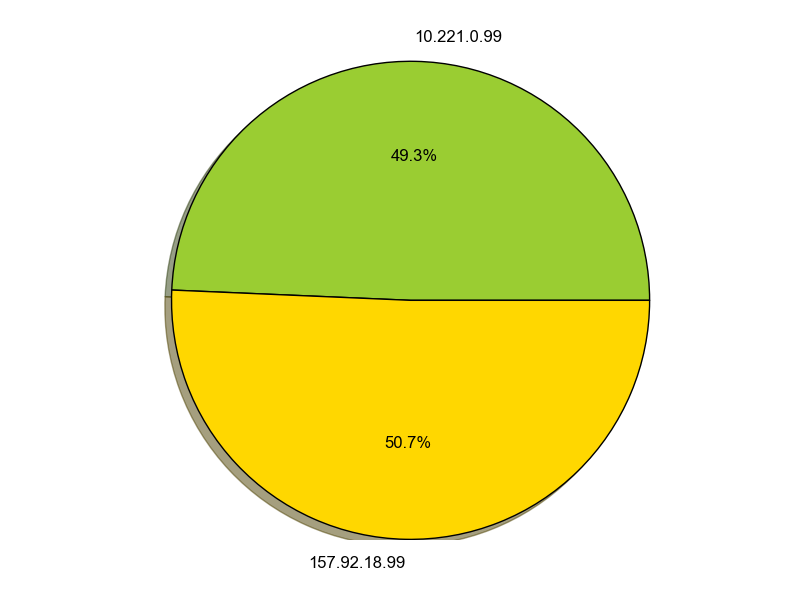
\includegraphics[width=12cm]{imgs/outputPabloRedAulasPab2_p-arp_is_src-torta.png}
		\caption{is-at SRC Red Aulas Biblioteca del Pabellón 2 FCEyN}
	\end{figure}
\end{center}



% Para mi con el de arriba alcanza y sobra.
% --Ok(Nicolasso)
% \begin{center}
% 	\begin{figure}[ht]
%     	\centering
% 		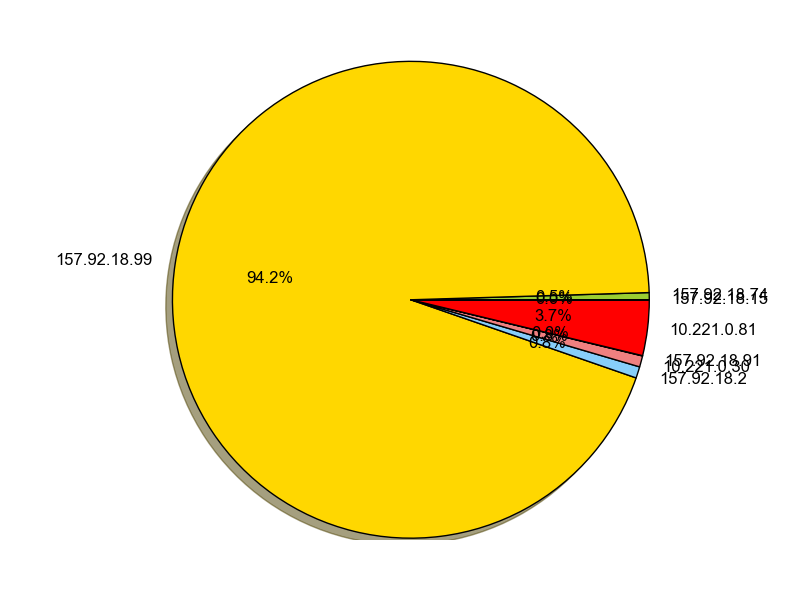
\includegraphics[width=12cm]{imgs/outputPabloRedAulasPab2_p-arp_who_src-torta.png}
% 		\caption{Who-Has SRC Red Aulas Biblioteca del Pabellón 2 FCEyN}
% 	\end{figure}
% \end{center}

\begin{center}
	\begin{figure}[ht]
    	\centering
		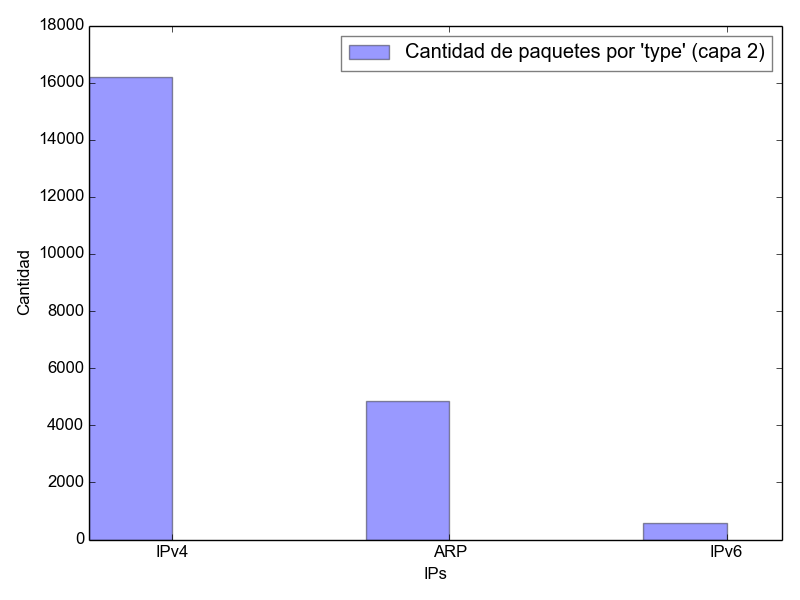
\includegraphics[width=12cm]{imgs/outputPabloRedAulasPab2_p-pkgs_by_type.png}
		\caption{Cantidad de paquetes por Tipo Red Aulas Biblioteca del Pabellón 2 FCEyN}
	\end{figure}
\end{center}





\FloatBarrier
\newpage
\subsection{Starbucks}

Se realizó una captura de 30 minutos en la red pública provista por el local Starbucks del lugar. El primer fenómeno que se pudo observar fue una alta aparición de la IP 10.254.54.1 en el campo destino de los paquetes ARP Who-Has, lo que a su vez nos indica que es el símbolo que brinda menor información, por lo que inferimos que debe tratarse del router. En la figura 8 puede observarse que el 51\% de los paquetes Who-Has tienen como destino dicha IP y en la figura 9 puede verse que se alcanzaron a contabilizar 60 de ellos, mientras que a otros destinos no se alcanzan a contar 10.

\FloatBarrier
\begin{center}
	\begin{figure}[ht]
    	\centering
		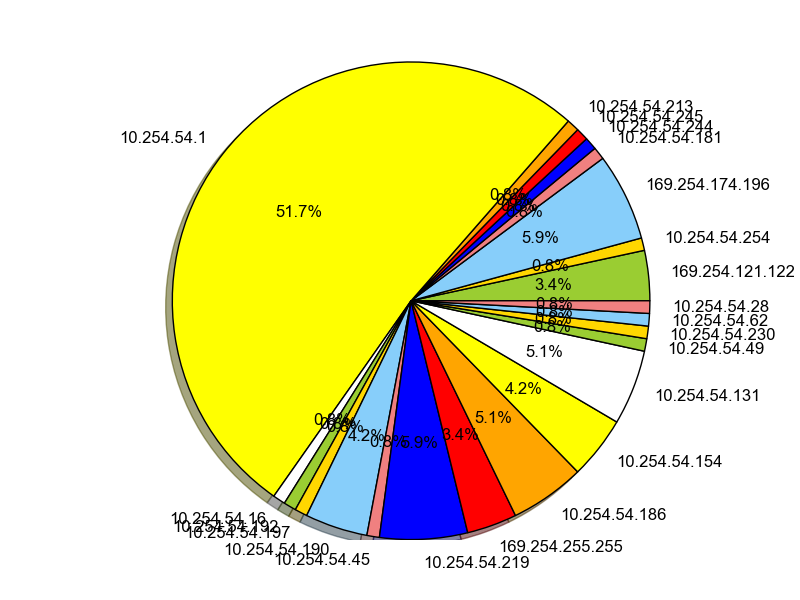
\includegraphics[width=11cm]{imgs/output_robert_starbucks_24-04-2015_p-arp_who_dst-torta.png}
		\caption{Who-Has DST Red Starbucks}
	\end{figure}
\end{center}
\FloatBarrier
\begin{center}
	\begin{figure}[ht]
    	\centering
		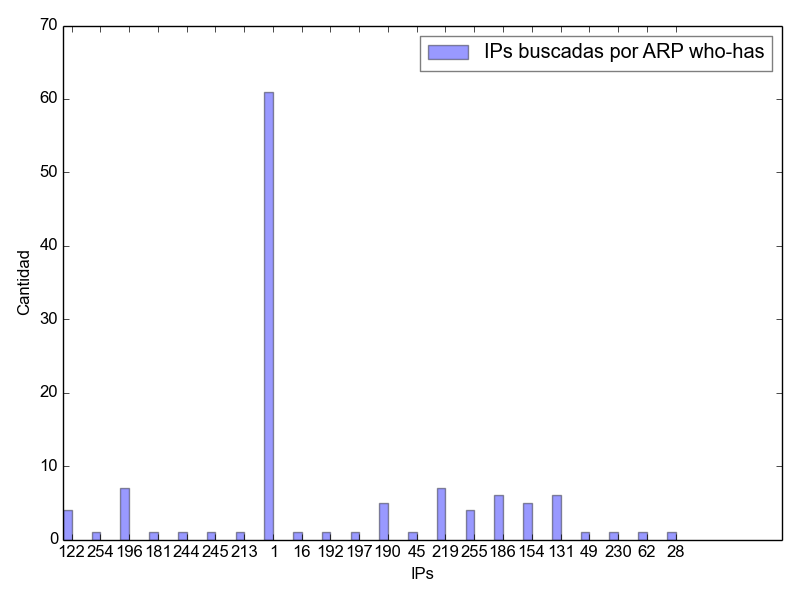
\includegraphics[width=11cm]{imgs/output_robert_starbucks_24-04-2015_p-arp_who_dst.png}
		\caption{Who-Has DST Red Starbucks}
	\end{figure}
\end{center}
\FloatBarrier

\newpage
Adicionalmente podemos ver en las figuras 10 y 11 que dicha IP también aparece de forma distinguida como origen de esos paquetes. Pero también podemos observar otro fenómeno, la aparición de la IP 0.0.0.0. como origen de una cantidad importante de paquetes. Esto ocurre cuando un cliente que se conecta a una red que posee un servidor DHCP. 

\FloatBarrier
\begin{center}
	\begin{figure}[ht]
    	\centering
		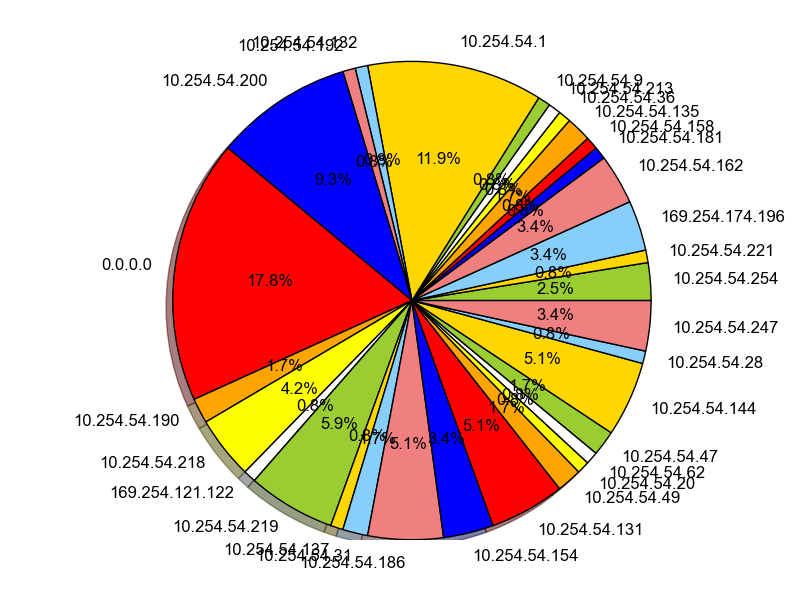
\includegraphics[width=11cm]{imgs/output_robert_starbucks_24-04-2015_p-arp_who_src-torta.png}
		\caption{Who-Has SRC Red Starbucks}
	\end{figure}
\end{center}
\FloatBarrier
\begin{center}
	\begin{figure}[ht]
    	\centering
		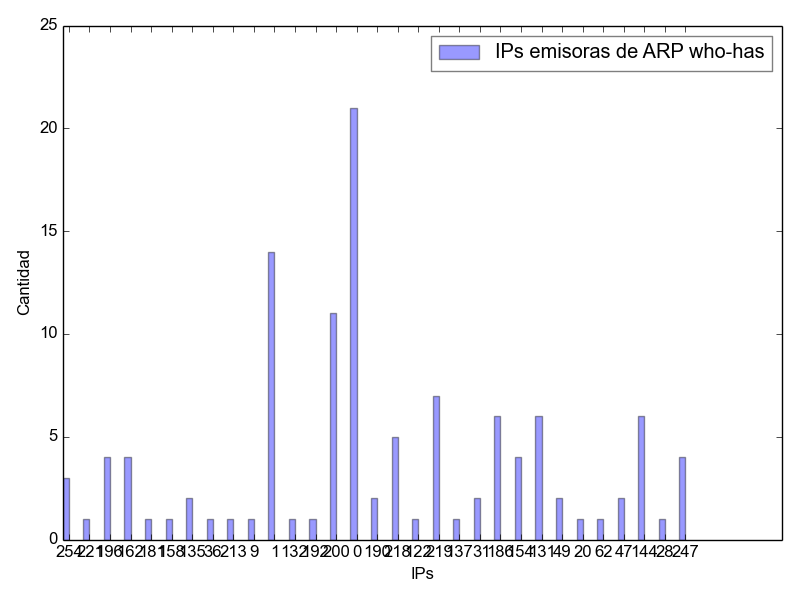
\includegraphics[width=11cm]{imgs/output_robert_starbucks_24-04-2015_p-arp_who_src.png}
		\caption{Who-Has SRC Red Starbucks}
	\end{figure}
\end{center}
\FloatBarrier

\newpage
Cuando el cliente solicita una IP de éste, manda una petición por broadcast con su ID para que lo detecte el servidor. Una vez detectado éste manda una o varias ofertas de IP a ese ID. El cliente eventualmente podría recibir la oferta, tomar uno de esos IP y extraer la dirección del router. Pero como el servidor realiza la misma operación con todos los demás clientes que pidan una IP, el cliente debe comprobar que la IP que eligió no la tiene otro cliente. Para esto, envía un paquete who-has con su MAC address y la IP 0.0.0.0 como fuente para evitar confundir las ARP caches en otros hosts. Si el who-has es respondido, el cliente rechaza el IP elegido.

Es decir que la aparición de dichos paquetes es causada por clientes verificando las IP otorgadas por el servidor DHCP de la red.

~

Por último, entre los paquetes capturados detectamos varios que usaban el rango 169.254.0.0/16 como dirección IP origen o destino, el cual difiere con el rango utilizado para las IP asignadas por el servidor DHCP a los dispositivos de la red. Estas direcciones son llamadas ``direcciones de enlace local'' y son direcciones reservadas. Un host puede asignarse una IP libre de enlace local para acceder de forma básica a la red, permitiendo comunicarse con otros dispositivos de la red, pero no con dispositivos externos a la misma
\footnote{\url{http://es.wikipedia.org/wiki/Direcci\%C3\%B3n_de_Enlace-Local}}.

\clearpage
\newpage
\subsection{LAN Laboratorios de Computación del Pabellón 1 FyCEN}

\indent Los siguientes gráficos corresponden a la red de los laboratorios de computación del pabellón 1.

%El de más abajo deja a un nodo más en evidencia. Asumamos que es el router y ya :p
% \begin{center}
% 	\begin{figure}[ht]
%     	\centering
% 		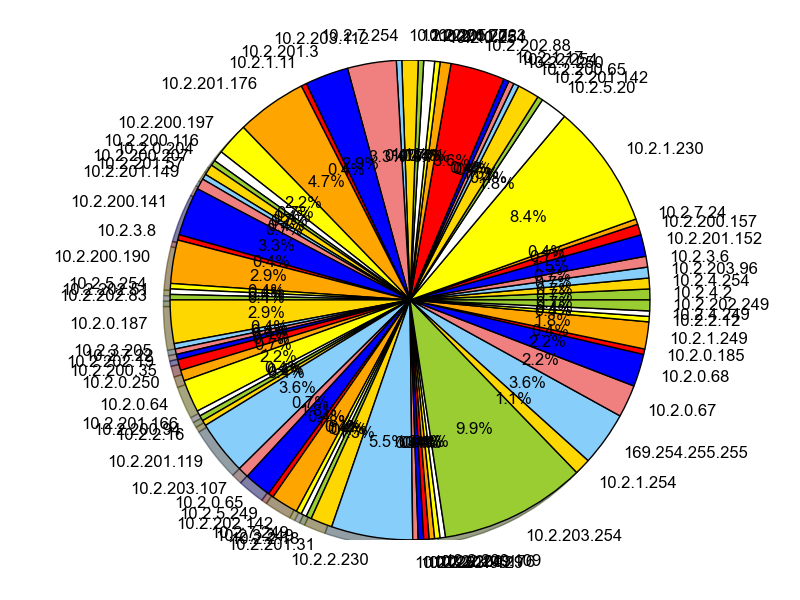
\includegraphics[width=12cm]{imgs/output_laski_labos_p-arp_who_dst-torta.png}
% 		\caption{Who-Has DST Red Laboratorios de Computación Pabellón 1}
% 	\end{figure}
% \end{center}


\begin{center}
	\begin{figure}[ht]
    	\centering
		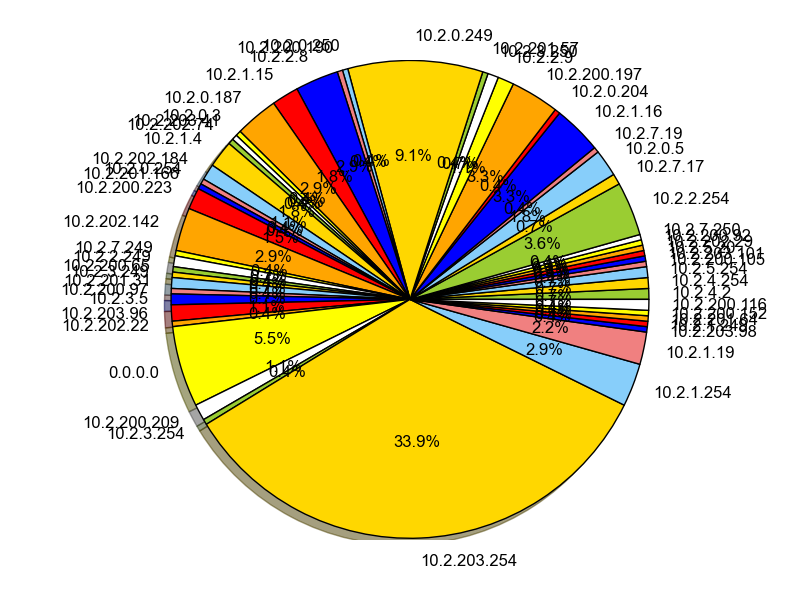
\includegraphics[width=12cm]{imgs/output_laski_labos_p-arp_who_src-torta.png}
		\caption{Who-Has SRC Red Laboratorios de Computación Pabellón 1}
	\end{figure}
\end{center}

\indent En este gráfico se pueden observar entre los nodos distinguidos a los que tienen la IP:
\begin{itemize}
	\item \textit{10.2.203.254}. Este siendo el más distinguido, se supuso al comienzo como el Gateway de la red wifi. Más adelante esto se pudo corroborar al consultarlo con el administrador de dicha red.
    \item \textit{10.2.0.249}. Se piensa que al distinguirse bastante contra el resto, este puede ser o bien una computadora que está generando mucho tráfico o quizás la impresora de los laboratorios la cual puede ser solicitada por muchos nodos diferentes.
    \item \textit{0.0.0.0}. Al igual que como está explicado en la sección anterior, en esta LAN también sucede que se inicializan los nodos que se quieren attachear a la red hasta que se les asigna una IP.
\end{itemize}


\FloatBarrier
\begin{center}
	\begin{figure}[ht]
    	\centering
		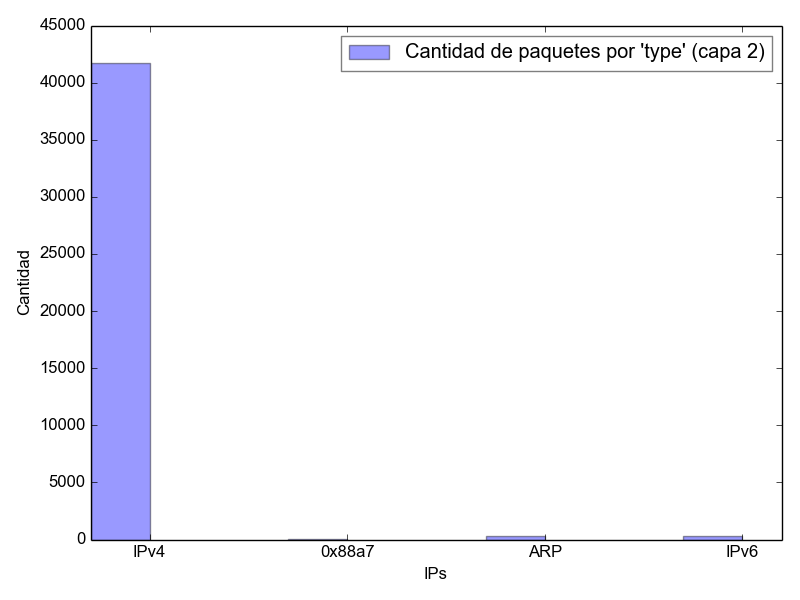
\includegraphics[width=12cm]{imgs/output_laski_labos_p-pkgs_by_type.png}
		\caption{Cantidad de paquetes por tipo Red Laboratorios de Computación Pabellón 1}
	\end{figure}
\end{center}

En este gráfico podemos observar la distribución de paquetes en función del tipo.
El caso particular de esta red nos permitió observar un tipo de paquete que desconocíamos: $0x88a7$. Este número resultó estar asociado a un protocolo llamado ``Cluster protocol''. No parecía ser muy difundido, ya que no figuraba en la lista de EtherTypes de Wikipedia\footnote{http://en.wikipedia.org/wiki/EtherType} y encontramos reportes de que WireShark no lo soportaba.
Por lo demás, el tráfico sigue una distribución similar a la esperada en base a lo ya explicado en experimentos anteriores.

\FloatBarrier





\clearpage

\section{Conclusiones}
En el trabajo práctico trabajamos analizando las rutas que siguen los paquetes para llegar a distintos destinos de nuestro interés. Para lograr dicho objetivo, desarrollamos una herramienta que realiza un echo request al destino pero incrementando el valor TTL del paquete ICMP de a una unidad. De esta forma los distintos hosts que el paquete transita nos devuelven un \textit{Time Exceeded} como respuesta junto con su IP, haciendo posible, además de su identificación y un orden de los mismos, un calculo de RTT. Midiendo diferencias significativas en el valor de RTT logramos identificar los enlaces submarinos que conectan al mundo entre sí.

En el intento de medir hasta que host llega el paquete ICMP con determinado TTL o si llega a destino, nos encontramos con que algunos de los hosts no respondían nada. Esto resulta de la configuración de los mismos que por medidas de seguridad no permiten, o bien responder paquetes o bien filtran paquetes ICMP. Estos hosts no fueron incluidos en el analisis de las rutas y los RTT finales de cada Hop incluyen el tiempo que toma transitar por Hosts que no registran estos paquetes. Como conclusión a esto, hoy en día no se puede fiar del uso de los paquetes ICMP para realizar traceroutes dado que no todos los routers están configurados para tratar con ellos. Por esta razón, creemos que utilizar paquetes TCP sería de mayor precisión para obtener todos los hops de una ruta aunque habría que constatarlo experimentalmente.

Nos encontramos con resultados interesantes cuando analizamos los datos. Por ejemplo, cuando intentamos realizar la gelocalización de los distintos IPs. En ese caso, existen IPs que tienen un rango correspondiente a un país específico pero físicamente estan ubicados en otras regiones del mundo, lo que dificultó la ubicación de los mismos y la creación de los distintos mapas. Por otro lado, mediante la detección de cambios de ruta, pudimos observar que países como India tienen una alta redundancia en sus rutas (o un problema en su red), ya que se detectaron muchos cambios de rutas al realizar las repeticiones. Ademas, notamos que habian muchas universidades que no responden a un echo-request (por ejemplo la Universidad de Tokyo, Japón) por lo que se dificultó su selección.

Por otro lado, pudimos comprobar empíricamente la relación proporcional entre el RTT y la distancia geográfica de las rutas, y su relación inversa con el valor estimado por el throghput obtenido por la ecuación de Mathis, salvando algunas inconsistencias menores.

Descubrimos diferentes incosistencias entre las tablas de geolocalización IP, y tuvimos que tomar información de varias hasta encontrar datos consistentes con nuestros resultaods.

En un trabajo futuro, sería buena idea analizar las distintas rutas que puede tomar un paquete para llegar a destino, exponiendo los lugares por los que transita y los tiempos de cada uno de los caminos. También queda pendiente realizar este mismo análisis y otros utilizando paquetes TCP para mayor precisión.


\end{document}















